\sektion{11}{Balanced Trees}
\subsektion{Abstract}
In this chapter we describe two programming projects that involve trees. The projects in question are improvements of the classes mentioned earlier in the text: the priority queue (pg. 433 Proj. 5) and the set class (similar to the bag class). We will also analyze the time performance of tree algorithms.
\subsektion{Heaps}
\subsubsektion{The Heap Storage Rules}
A heap is a binary tree where a less than operator forms a \emph{strict weak ordering}\footnote{For a reminder of the rules for strict weak ordering, see pg. 139} that can be used to compare the nodes' entires.

\subsubsektion{Heap Storage Rules}
A heap is a binary tree where the entries of the nodes can be compared with the less-than operator of a stricct weak ordering. In addition, these two rules are followed:
\begin{enumerate}
\item The entry contained by a node is never less than the entries of hte node's children
\item The tree is a complete binary tree, so that every level except hte deepest must contain as many nodes as possible; and at the deepest level, all the nodes are as far left as possible.
\end{enumerate}
\begin{figure}[h]
\centering
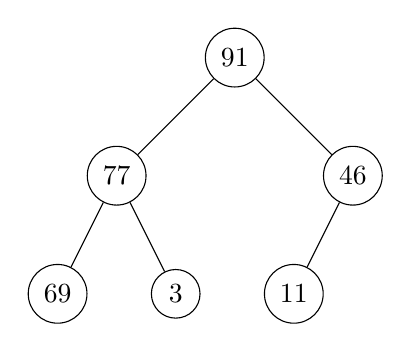
\begin{tikzpicture}[level distance=1.5cm,
  level 1/.style={sibling distance=3cm},
  level 2/.style={sibling distance=1.5cm}]
\node[circle,draw]{$91$}
    child{
        node[circle,draw]{77}
            child {
                node[circle,draw]{69}
            }
            child{
                node[circle,draw]{3}
            }
    }
    child {
        node[circle,draw]{46}
            child {
                node[circle,draw]{11}
            }
            child[missing]{}
        };
\end{tikzpicture}
\caption{An example of a heap}
\end{figure}
\emph{Should we know the size of the heap we wish to implement, the most effective implementation can use a fixed-size array.}
\subsubsektion{The Priority Queue with Heaps}
The difference between a queue and a priority queue is that the elements in a priority queue can be compared with the othe rentries using a $<$ operator. When entries leave a priority queue, the highest priority entries always leave first.

In a heap implementation of the priority queue, each node of the heap contains one entry. The tree is maintained so that it follows the heap storage rules using the entries' priorities to compare nodes. In this way the entry contained by a node is never less than the entries of the node's children and the tree is a complete binary tree.

We'll focus on two operations: adding a new entry and removing an entry with the highest priority.
\subsubsektion{Adding an Entry to a Heap}
For our purposes we will use a heap made of integers with no overloaded infix operators. Furthermore, suppose we have the following heap:

\begin{figure}[h]
\centering
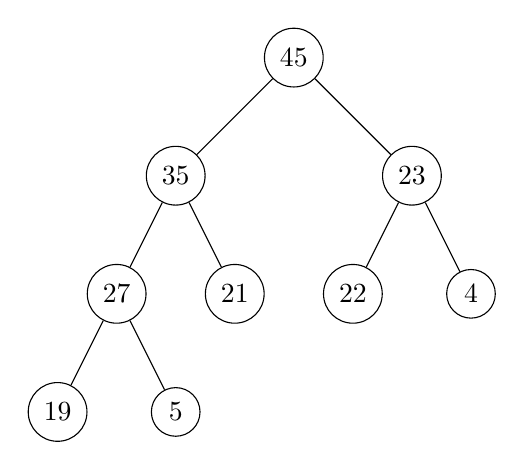
\begin{tikzpicture}[level distance=1.5cm,
  level 1/.style={sibling distance=3cm},
  level 2/.style={sibling distance=1.5cm}]
\node[circle,draw]{$45$}
    child{
        node[circle,draw]{35}
            child {
                node[circle,draw]{27}
                    child {
                        node[circle,draw]{19}
                    }
                    child {
                        node[circle,draw]{5}
                    }
            }
            child{
                node[circle,draw]{21}
            }
    }
    child {
        node[circle,draw]{23}
            child {
                node[circle,draw]{22}
            }
            child {
                node[circle,draw]{4}
            }
        };
\end{tikzpicture}
\caption{A basic heap}
\end{figure}
Suppose we want to add the entry 42, to keep the completeness of the binary tree we will insert it to the left child node of 21.

\begin{figure}[h]
\centering
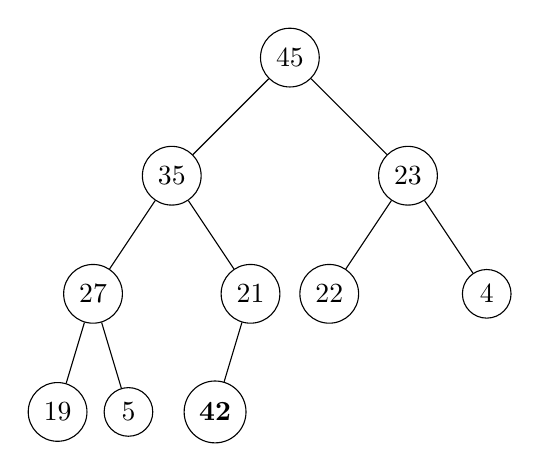
\begin{tikzpicture}[every node/.style={circle,draw},
  level 1/.style={sibling distance=30mm},
  level 2/.style={sibling distance=20mm},
  level 3/.style={sibling distance=9mm}]
\node[circle,draw]{$45$}
    child{
        node {35}
            child {
                node {27}
                    child {
                        node {19}
                    }
                    child {
                        node {5}
                    }
            }
            child{
                node {21}
                    child {
                        node {\textbf{42}}
                    }
                    child[missing]{}
            }
    }
    child {
        node {23}
            child {
                node {22}
            }
            child {
                node {4}
            }
        };
\end{tikzpicture}
\caption{Inserting 42}
\end{figure}

\begin{figure}[h]
\centering
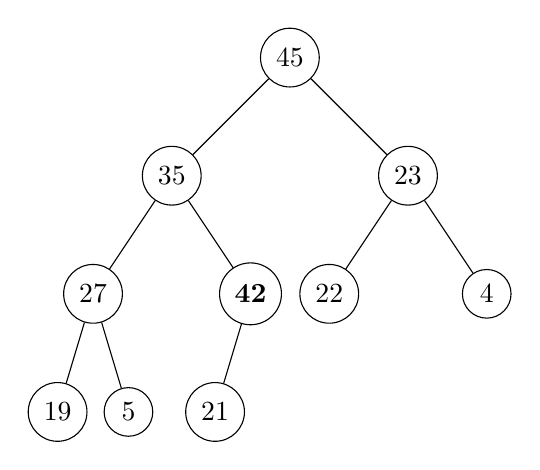
\begin{tikzpicture}[every node/.style={circle,draw},
  level 1/.style={sibling distance=30mm},
  level 2/.style={sibling distance=20mm},
  level 3/.style={sibling distance=9mm}]
\node[circle,draw]{$45$}
    child{
        node {35}
            child {
                node {27}
                    child {
                        node {19}
                    }
                    child {
                        node {5}
                    }
            }
            child{
                node {\textbf{42}}
                    child {
                        node {21}
                    }
                    child[missing]{}
            }
    }
    child {
        node {23}
            child {
                node {22}
            }
            child {
                node {4}
            }
        };
\end{tikzpicture}
\caption{Re-balancing the heap.}
\end{figure}

\begin{figure}[h]
\centering
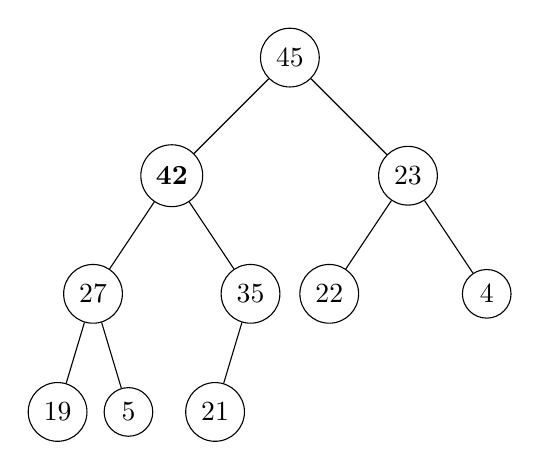
\begin{tikzpicture}[every node/.style={circle,draw},
  level 1/.style={sibling distance=30mm},
  level 2/.style={sibling distance=20mm},
  level 3/.style={sibling distance=9mm}]
\node[circle,draw]{$45$}
    child{
        node {\textbf{42}}
            child {
                node {27}
                    child {
                        node {19}
                    }
                    child {
                        node {5}
                    }
            }
            child{
                node {35}
                    child {
                        node {21}
                    }
                    child[missing]{}
            }
    }
    child {
        node {23}
            child {
                node {22}
            }
            child {
                node {4}
            }
        };
\end{tikzpicture}
\caption{Re-balancing the heap.}
\end{figure}
\newpage
\subsubsektion{Removing an Entry from a Heap}
When an entry is removed from a priority queue, we must always remove the entry with the highest priority. Consider the following tree, the root of the tree will be removed since it has the highest priority.

\subsubsektion{Pseudocode for Adding and Removing Entries}
\begin{enumerate}
\item Place a new entry in the heap in the first available location.
\item \emph{while} (the new entry's parent is less than hte new entry): swap the new entry with its parent.
\end{enumerate}

\begin{enumerate}
\item Copy the entry at the root of the heap to the variable that is used to return a value.
\item Copy the last entry in the deepest level to the root, and then take this last node out of the tree.
\item \emph{while} (the out of place entry is less than one of its children): swap the out of place entry wits highest child.
\end{enumerate}

\subsektion{B-Trees}
Section 10.5 implements the bag class with binary search trees, however their efficiency can sometimes go awry. We will analyze the problem and show one way to fix it.
\subsubsektion{The Problem of Unbalanced Trees}
Let's assume that we have a binary tree that's left-aligned and populated with the values 1 through 5. This is troublesome since this implementation is essentially no better than a linked list; continue adding values to the left branch of the tree and the problem exacerbates. We can solve this problem in several ways, for example we could periodically balance the search trees (explained in Ch.10 pg.538). Another method is to use a B-Trees, where the leaves cannot become deep (relative to the number of nodes).
\subsubsektion{The B-Tree Rules}
Every B-Tree depends on a positive constant integer $MINIMUM$ which serves as the number of entries held in a single node.
\begin{itemize}
\item The root may have as few as one entries while every other node has at least $MINIMUM$ entires.
\item The maximum number of entries in a node is twice the value of $MINIMUM$.
\item The entries of each B-Tree node are stored in a partially filled array, sorted from smallest to largest.
\item The number of subtrees $n$ below a nonleaf node is always $n=m+1$ where $m$ is the number of entires in the node.
\end{itemize}
\begin{example}\label{example:numsubtrees}
Consider a node that has 42 entries. This node will have 43 children according to our prevoius statement. Each subtree will be referred to as subtree 0, subtree 1,$\cdots$, subtree 42.
\end{example}
\begin{itemize}
\item For any nonleaf node the subtrees are ordered from least to greatest value
\end{itemize}
\begin{example}
Consider a nonleaf node that contains two integer entries 93 and 107. This nonleaf node must have three child nodes based upon example \ref{example:numsubtrees}. subtree0 must be less than the value 93, subtree1 must have a value between 93 and 107, and subtree2 must be greater than 107.
\end{example}
\begin{itemize}
\item Every leaf in a B-Tree has the same depth.
\end{itemize}
\subsubsektion{The Set ADT with B-Trees}
The rest of this section discusses methods for implementing B-Trees. I will refer to the text as much as possible to avoid typing out huge chunks of code.

\subsubsektion{Invariant for the Set Class Implemented with a B-Tree}
\begin{enumerate}
\item The items of the set are stored in a B-Tree that comply with the aforementioned rules.
\item The number of entries in the tree's root are stored in the member variable data\_count. The number of subtrees of the root is stored in the member variable child\_count.
\item The root's entries are stored in data[0] through data[data\_count-1].
\item If the root has subtrees, then these subtrees are stored in sets pointed to by the pointers subset[0] through subset[child\_count-1].
\end{enumerate}

\subsubsektion{Searching for an Item in a B-Tree}
The set class (defined on pg. 551) has a member function (count) that determines whether an item called $target$ appears in the set. Remember that count always returns 0 if $target$ is not found, and 1 if it is.

We search B-Trees in much the same way we search binary search trees. The basic algorithm is as follows:
\begin{itemize}
\item Check the root, if $count=1$ then we're done!
\item If the root has no children, the search is also done.
\item Make a recursive call to the children to check for $target$
\end{itemize}
We justify the recursive call by arguing that the subset of the root \emph{has} to be smaller than the entire set.

\subsubsektion{Inserting an Item into a B-Tree}
The $insert$ member function defined in the set class adds a new item to the B-Tree. We'll attempt to implement a loose insertion which \emph{may} result in an illegal tree.

\subsubsektion{The Loose Insertion into a B-Tree}
Our initial condition is that the B-Tree is valid. Our postconditions are as follows:
\begin{itemize}
\item If the value is already set, leave the B-Tree unchanged.
\item Otherwise add the entry to the set. The B-Tree remains valid, however it's possible that the number of entries in the root of the set may be higher than $MAXIMUM$.
\end{itemize}
So a basic algorithm for this insertion seems fairly straightforward, and begins much like the search algorithm: find the location of the root's entires that is not less than the new entry.
\begin{itemize}
\item Set local variable $i$ equal to the first index, such that data[$i$] is less than the entry.
\item If we find the value of $i$ at data[$i$] return; there's nothing to do!
\item If the root has no children, add a new entry to the root.
\item Otherwise, save the value from the recursive call subset[$i$]$\to$loose\_insert(entry); 
\end{itemize}

\subsubsektion{A Private Member Function to Fix an Excess in a Child}
To fix a child with $MAXIMUM+1$ entries, the child node is split into two nodes that each contain $MINIMUM$ entries. This leaves one extra entry, which is passed upward to the parent.

\subsubsektion{Back to the Insert Member Function}
By using the loose insertion function defined above, we have only two steps to ensure a smooth insertion.
\begin{enumerate}
\item If loose insert returns false, we have nothing to do.
\item Otherwise, if the maximum value has been exceeded for the root, fix the tree with out fix\_excess function.
\end{enumerate}
The last step can be performed in two parts. We first copy all the pointers of the child nodes and clear the root, essentially bumping the whole tree down one node. We've changed the scope of the problem to our old root, and this is much simpler to fix. We split the old root node into a subset and shift the middle value up to our new root. Refer to page 562 for a pictoral representation of this shift.

\subsubsektion{Employing top Down Design}
Essentially, top down design means we implement functions in such a way that each successive function call solves a smaller and smaller problem. Through this methodology it becomes easier to determine points of failure.

\subsubsektion{Removing an Item from a B-Tree}
The $erase$ member function of the set removes an entry from the B-Tree. Most of the work is accomplished with a private member function: $loose\_erase$ (think $loose\_insert$). A simple algorithm for loosely removing a value from a tree looks something like this:
\begin{itemize}
\item If $target$ does not exist, there's nothing to do
\item If we found $target$ and it has children, fix the root of the entire tree so that it no longer has zero entries.
\end{itemize}

\subsubsektion{The Loose Erase from a B-Tree}
\begin{itemize}
\item Make a local variable $i$ equal to the first index at data[$i$] that is not less than $target$.
\item Deal with one of four possibilities
\begin{enumerate}
    \item The root has no children and we did not find $target$. Nothing to do.
    \item The root has no children and we found the $target$. Remove $target$.
    \item The root has children and we did not find $target$.
        \begin{itemize}
            \item Make a recursive call to the child subsets.
            \item Call a private member function $fix\_shortage$ to  validate the B-Tree.
        \end{itemize}
    \item The root has children and we did find $target$.
        \begin{itemize}
            \item Instead of removing $target$ we will remove the largest item in hte subset.
            \item Take a copy of this largest item and place it into data[$i$] which contains the target.
            \item The total effect is the same as removing $target$.
        \end{itemize}
\end{enumerate}
\end{itemize}
\subsubsektion{A Private Member Function ot Fix a Shortage in a Child}
\begin{example}[Transfer extra entry from subset${[} i-1 {]}$]
Suppose that subset[$i-1$] has more than the min. number of entries.
\begin{itemize}
\item Transfer data[$i-1$] down to the front of subset[$i$]$\to$data.
\item Transfer the final item of subset[$i-1$]$\to$data up one to replace data[$i-1$].
\item If subset[$i-1$ has children, transfer the final child of subset[$i-1$] over to the front of subset[$i$].
\item Consult the example provided on page 567 for a pictoral representation of this method.
\end{itemize}
\end{example}
\begin{example}[Transfer extra entry from subset${[} i+1 {]}$] Compliment the method described in Case 1.
\end{example}
\begin{example}[Combine subset${[} i {]}$ w/ subset${[} i-1 {]}$]
Suppose that $i > 0$ but it only has $MINIMUM$ entries.
\begin{enumerate}
\item
    \begin{itemize}
    \item Transfer data[$i-1$] down to the end of subset[$i-1$]$\to$data, which removes the item from the root.
    \item Shift data[$i$], data[$i+1$], and so on, leftward.
    \item Subtract 1 from data\_count and add one to subset[$i-1$]$\to$data\_count.
    \end{itemize}
\item
    \begin{itemize}
    \item Transfer all items and children from the current subset to the end of subset[$i-1$]
    \end{itemize}
\item
    \begin{itemize}
    \item Delete the node subset[$i$] and shift subset[$i+1$], subset[$i+2$], and so on, leftward.
    \end{itemize}
\end{enumerate}
\end{example}
\begin{example}[Combine subset${[} i {]}$ w/ subset${[} i+1 {]}$]
\begin{itemize}
Implement the compliment of the previous example.
\end{itemize}
\end{example}
\subsubsektion{Removing the Biggest Item from a B-Tree}
Removing the biggest item is simple if the root has no children. We simply copy the last item of data into the reference parameter. If the root has children, we make a recursive call to remove the largest entry from the rightmost child.


